\section{Qt}
\begin{minipage}{17cm}
	Qt (sprich cute =süess) ist eine plattformübergreifende Programmierungsapplikation für grafische Benutzeroberflächen (GUI = Graphical User Interface).\\
	Qt wurde 1991 gegründet und gehörte der Firma Trolltech. Im Jahr 2008 übernahm Nokia die Firma Trolltech. Im Jahr 2014 wurde Qt als Open-Source-Projekt verwaltet. 
\end{minipage}
\begin{minipage}{1.5cm}
	
\includegraphics[width=1.5cm]{images/qt_logo.jpg}
\end{minipage}

\subsection{Grundlagen zu Qt}
\begin{minipage}{8cm}
	\begin{itemize}
		\item Qt C++ Klassenbibliothek stellt GUI-Elemente zur Verfügung
		\item Das GUI wird als C++ Sourcefile geschrieben
		\item Standartklasse QtGui und QtCore werden automatisch inkludiert
		\item Alle Qt Widgets werden auf dem Heap erstellt
		\item Jedes Programm enthält eine Instanz von QApplication
		\item QApplication hält alles zusammen
		\item siehe Hello World Beispiel im Anhang für näheres
	\end{itemize}
\end{minipage}
\begin{minipage}{10cm}
	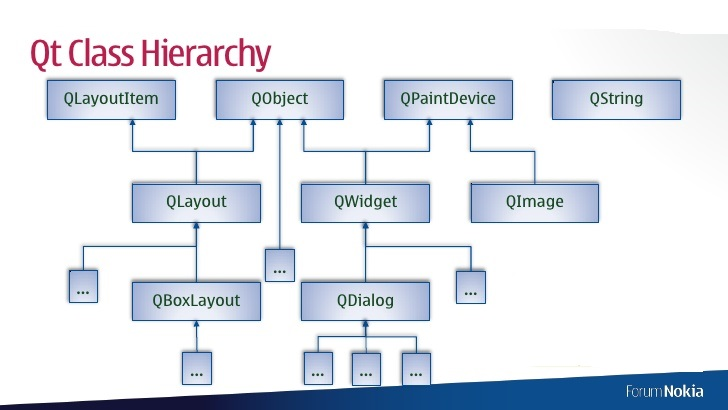
\includegraphics[width=10cm]{images/qt_classes.jpg}
\end{minipage}

\begin{multicols}{2}
	\subsubsection{QObject}
	\begin{itemize}
		\item QObject ist die Basisklasse des Qt-Modells
		\item stellt das Memorymanagement (automatische delete) für alle abgeleitet Klassen von QObject zur Verfügung. Es entstehen Objektbäume. 
		\item stellt die connect-Funktion zur Verfügung
		\item bearbeitet das Eventhandling
		\item hat keine visuelle Representation
	\end{itemize}
	
	\subsubsection{Qt Building}
	\begin{itemize}
		\item qmake Makefile-Generator
		\item macht aus plattformunabhängiem Projektfile (.pro) ein plattformspezifisches Projektfile. 
		\item die gewünschte Plattform wird qmake als Option mitgegeben
		\item Bei Build-Problemen alle Dateien ausser .pro und Sourcefile löschen
	\end{itemize}
\end{multicols}

\subsubsection{Qt Konvention}
\begin{tabular}{|l|l|l|}
	\hline \textbf{Was} & \textbf{Beispiel} &\textbf{Konvention}\\
	\hline Qt-Modulname & "QtCore"& \textit{Qt}\\
	\hline Qt-Klassenname & "QString" & \textit{Q}\\
	\hline Qt-Variablen-,Funktionsname & "qTranslator, qDebug()"& \textit{q}\\
	\hline Qt-include & "\#include <QtGui>& \textit{ohne.h}\\
	\hline
\end{tabular}

\subsection{QWidget}
\begin{itemize}
	\item abgeleitet von QObject
	\item Eine Instanz der Klasse stellt eine grafisches Element dar
	\item Diese Klasse hat viele Methoden um Aussehen, Grösse, Position etc. zu verändern
	\item mit show() wird das Widget angezeigt, mit hide() wird das Widget versteckt
	\item Jedes Widget wird einem \textit{"Parent-Widget"} (Eltern) zugewiesen, ein solches Widgets nennt man dann \textit{Child-Widgets}
	\item Durch die Parent-Child Funktion entsteht eine Verschachtelung
	\item Ein Widget ohne Parent ist ein Top-Level-Widget oder Window	
	\item Das \textit{"Parent-Widget"} übernimmt Verwaltungsfunktionen wie Memory-Management, weiterleiten von Ereignisse an \textit{"Child-Widget}, anzeigen, verstecken von Widgets etc.
\end{itemize}

\begin{multicols}{3}
\subsubsection{Top-Level-Widget}
Die \textit{"Top-Level-Window"} sind Widgets welche auf der obersten Hierarchiestufe liegen. Sie haben keine \textit{"Parent-Widget"}.
Übliche Widgets für \textit{"Top-Level-Window"}: 
\begin{itemize}
	\item QMainWindow $\rightarrow$ Applikations-Window (Hauptfenster)
	\item QDialog $\rightarrow$ Popup-Window für Abfragen (Wirklich löschen), Hauptanwendung bleibt blockiert
	\item QWidget $\rightarrow$ Einfaches Fenster
\end{itemize}

\subsubsection{Parent-Child-Widgets}
\begin{itemize}
	\item Jedes QObject kann maximal ein Eltern-QObject haben
	\item Jedes QObject kann beliebig viele Kind-QObject haben
	\item Kind muss Eltern über sich informieren
	\item Entweder über Konstruktor, label->setParent(mainwindow) oder Layout Manager
\end{itemize}

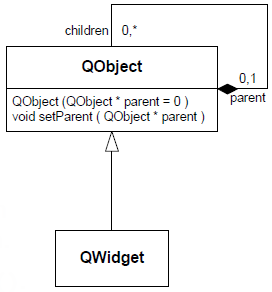
\includegraphics[width=5cm]{images/qt_parent_child.png}
\end{multicols}


\subsection{GUI-Programmierung}
Es gibt zwei grundlegende Aufgaben bei der GUI-Programmierung.\\
Das \textbf{Layout} legt Anordnung, Grösse  und Farbe fest.\\
Die \textbf{Interaktion} legt die Reaktion des Programmes auf eine Eingabe fest. \\

\subsection{Layout}
Es gibt drei Varianten wie Widgets innerhalb eines Widget angeordnet werden können, absolute Positionierung, Layout Manager und GUI-Designer (Qt Designer)

\subsubsection{Absolute Positionierung}
Mittels Methoden.
\begin{multicols}{2}	
	\lstinputlisting{source/Qt/methoden.cpp}
	
	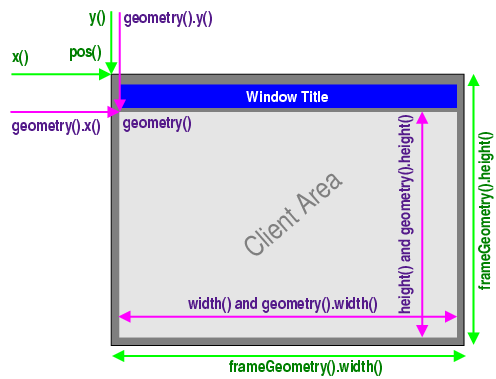
\includegraphics[width=8cm]{images/geometry.png}
\end{multicols}

\subsubsection{Layout Manager}
	\begin{tabular}{|l|l|}
		\hline \textbf{Klasse} & \textbf{Ort}\\
		\hline QVBoxLayout & Elemente vertikal\\
		\hline QHBoxLayout & Elemente horizontal\\
		\hline QGridLayout & zweidimensionales Gitter\\
		\hline QFormLayout & Elemente zeilenweise\\
		\hline QStackedLayout & aufeinandergelegt\\
		\hline
	\end{tabular}
	
\subsubsection{GUI-Designer / Qt Designer}	
	Anordnung innerhalb eines Formulars mittels interaktiven Tools, anschliessend Umwandlung in Code. 	

\subsection{Interaktion}
In Qt werden die Eingaben als SIGNALS bezeichnet und die Ausgaben als SLOTS. Mittels der Funktion connect() werden die beiden miteinander verknüpft.\\
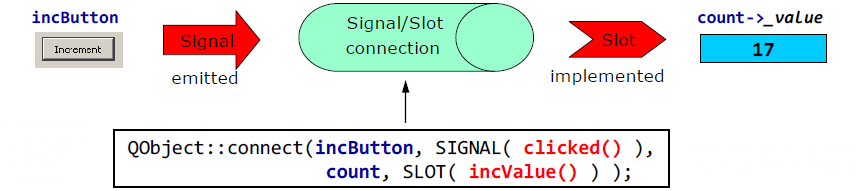
\includegraphics[width=15cm]{images/connect.png}

\begin{multicols}{3}
\subsubsection{SIGNALS}
\begin{itemize}
	\item nur deklariert, nie definiert
	\item kein Zugfriffsrecht vergeben
	\item Rückgabetyp immer void
\end{itemize}

\subsubsection{SLOTS}
\begin{itemize}
	\item deklariert und definiert
	\item oftmals Memberfunktion, auch normal abrufbar
	\item Zugriffsrechte
\end{itemize}

\subsubsection{connect}
\begin{itemize}
	\item Verbindungsfunktion zwischen Input und Output
	\item ein Signal zu mehreren Slots
	\item mehrere Signale zu einem Slot
\end{itemize}
\end{multicols}

\vspace{0.5pt}
\textbf{Beispiele connect-Funktion}
\lstinputlisting{source/Qt/connect.cpp}

\subsection{Zeichnen und Malen}
\begin{multicols}{2}
	\subsubsection{QPainter}
	Der Maler mit Mal-,\& Zeichenwerkzeugen.\\
	
	\begin{tabular}{|l|l|}
		\hline \textbf{Klasse} & \textbf{Werkzeug}\\
		\hline QPen & Zeichenstift\\
		\hline QBrush & Pinsel\\
		\hline QFont & Schriftart\\
		\hline draw & Formen malen\\
		\hline
	\end{tabular}
	
	\subsubsection{QPaintDevice}
	Oberfläche wo darauf gezeichnet \& gemalt werden kann
	QPainter-Objekte zeigen auf QPaintDevice-Objekte. QPaintDevice ist eine abstrakte Basisklasse welche nicht von QObject abgeleitet ist und daher \textbf{kein automatisches delete.}\\

\end{multicols}

\subsubsection{Vorgehen}
\lstinputlisting{source/Qt/qpainter.cpp}